\scanpage{13}
% archive sheet number: 12
5. \uline{Classe fondamentale locale}.

Reprenons l'homomorphisme de Gysin général (4.3), et notans que par la formule d'adjonction, sa connaissance équivaut à celle d'un homomorphisme
\[
f^{\handwritten{*}}(G)(d-d')\handwritten{[}2(d-d')\handwritten{]}\handwritten{\unsure{\longrightarrow|\Longrightarrow}}\mathrm{R}f^{\handwritten{!}}G,
\tag*{(4.4)}
\]
\margin{\handwritten{autre nom?}\begin{tikzpicture}[overlay,baseline]
\draw[gray,line width=.25pt] (0.12,0.35) .. controls (0.08,0.92) and (-0.60,0.82) .. (-1.12,0.58) .. controls (-1.78,0.30) and (-2.30,0.12) .. (-2.20,-0.18) .. controls (-2.04,-0.49) and (-1.50,-0.31) .. (-0.70,-0.05) .. controls (-0.20,0.12) and (0.22,0.20) .. (0.15,0.29);
\end{tikzpicture}}
\deleted{\unsure{qui, pour $f$}}\handwritten{[}On l'appelle l'homomorphisme \uline{classe fondamentale locale}(?)\handwritten{]}\handwritten{\unsure{/.|b}} Il est fonctoriel en $G$, et, comme nous avons vu au par.4, il suffit de le connaitre pour $G=A_Y$ pour le connaitre pour tout $G$. Dans ce cas, on peut l'interp\unsure{\deleted{é}r|\deleted{r}é}éter comme un homomorphisme
\[
\handwritten{\phi}_f:\quad A_X\handwritten{\longrightarrow}\mathrm{R}f^{\handwritten{!}}(A_Y)(d'-d)\ 2(d'-d)\handwritten{\unsure{,|)}}\quad
\begin{aligned}[b]
&\inserted{\handwritten{\text{i.e }}\handwritten{\varphi_f\in}\mathrm{H}^{\handwritten{2}(d-d')}(Y,\mathrm{R}f^{\handwritten{!}}(A_Y)(d-d'))}\\
&\deleted{\text{\unsure{sur|noté}}\ \unsure{\phi_Y|Y}}
\end{aligned}
\tag*{(4.5)}
\]
et il définit par suite une section, notée de même
\[
\begin{aligned}
&\deleted{\underline{\handwritten{\phi}}_f\ \handwritten{\unsure{\in|\leftarrow}}\ \mathrm{H}^0(Y,\underline{\mathrm{H}}^0\unsure{(}\mathrm{R}f^{\handwritten{!}}(A_Y)(d'-d)\ 2(d'-d))}\\
&\inserted{\handwritten{\varphi_f\in}\mathrm{H}^0(Y,\underline{\mathbb{R}}^{\handwritten{2}(d'-d)}\unsure{(\deleted{\unsure{\mathrm{R}}}|\deleted{(\unsure{\mathrm{R}}}}f^{\handwritten{!}}(A_Y))(d'-d))},
\end{aligned}
\tag*{(4.6)\begin{tikzpicture}[overlay,baseline]
\draw[gray,line width=.25pt] (-1.67,-1.06) .. controls (-1.39,-1.15) and (-1.50,-.84) .. (-1.59,-.52) .. controls (-1.72,-.10) and (-1.78,.13) .. (-1.58,.31) .. controls (-1.31,.53) and (-.86,.51) .. (-.51,.50) .. controls (-.13,.51) and (.16,.37) .. (.15,.24) .. controls (.14,-.08) and (.15,-.51) .. (.06,-.91) -- (.27,-.97);
\draw[line width=.4pt] (-1.57,-.67) .. controls (-1.43,-1.03) and (-1.47,-1.10) .. (-1.67,-1.06);
\draw[line width=.4pt] (.11,-.68) -- (.06,-.91) -- (.27,-.97);
\end{tikzpicture}}
\]
qu'on appelera également (et peut-être à meilleur escient) la \uline{classe fondamentale locale} \uline{pour} $f$. On notera que pour la connaitre pour tout $A$, il suffit de la connaitre pour les $\underline{\mathrm{Z}}/n\underline{\mathrm{Z}}$ (du moins si on se borne aux $A$ qui sont annulés par un même entier $n\handwritten{\geq}1$ premier aux car. résiduelles de $\unsure{\deleted{Y}S|\deleted{S}Y|\deleted{g}S|\deleted{S}g|\deleted{S}S}$): \deleted{La connaissance de (4.6) permet de réconstituer} plus précisément, la formation des clas\unsure{\deleted{s}e|\deleted{e}s}s $\handwritten{\phi}_f$ de (4.5) et de (4.6) est \uline{fonctoriel} en l'Anneau $A_S$ (voire, en $A_Y$).

Lorsqu'on dispose d'une ``formule de pureté''
\[
\deleted{\unsure{\underline{\mathrm{H}}^i(\mathrm{R}|\underline{\mathrm{H}}^i\mathrm{R}}}\ \mathrm{R}^i f^{\handwritten{!}}(A_Y)=0\quad\text{pour }i\handwritten{\unsure{<|\leq}}\unsure{\deleted{\mathrm{R}}2|\deleted{2}\mathrm{R}|\deleted{1}2|\deleted{2}1|\deleted{2}2}(d-d'),
\tag*{(4.7)}
\]
la connaissance de (4.6) équivaut même à celle de (4.5), ce dernier $\handwritten{\phi}_f$ méritant le nom de \uline{classe fondamentale globale} de $X$ sur $Y$.

Nous allons nous intéresser par la suite au c\unsure{\deleted{q}a|\deleted{a}q}s où $f:X\handwritten{\longrightarrow}Y$ e\unsure{s|\deleted{t}s|\deleted{s}t|\deleted{s}s}t une \uline{immersion fermée}. On sait alors que les formules de pureté (4.7)
